\lesson{7}{Oct 18 2021 Mon (22:03:53)}{Periodic Trends}{Unit 2}

\subsubsection*{Periodic Trends influenced by the Nuclear Charge.}

As the atomic number increases, the number of protons increases, too.
This trend is useful when searching for an element on the periodic table.
More massive elements (those with more protons and neutrons) will be
toward the bottom of the periodic table, and less massive elements will
be toward the top. But this is not the only useful pattern on the
periodic table. The periodic table shows many trends related to
the properties of elements and how they interact with one another.

\begin{marginfigure}
    \centering
    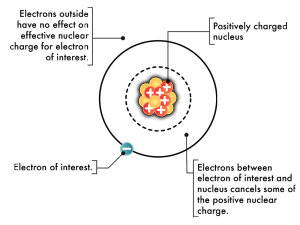
\includegraphics[width=\textwidth,height=\textheight,keepaspectratio]{images/effective-nuclear-charge}
    \sidecaption{In-detail look at an atom with a nuclear charge.}
    \label{fig:effective-nuclear-charge}
\end{marginfigure}

\paragraph{Effective Nuclear Charge} An atom with positively-charged nucleus surrounded by an electron cloud. The electrons closest to the nucleus provide a shield for the outer shell electron.

Charged particles like electrons are affected by electrostatic forces. Negatively charged electrons repel one another, and protons ($+$) and electrons ($-$) attract each other. So, the relative positions of electrons within an atom are influenced by the positive charge of the nucleus.

But not all electrons \bf{"feel"} the full positive charge of the nucleus. Electrons farthest from the nucleus are partially shielded by the electrons in the energy shells closer to the nucleus. So, outer shell electrons feel an effective nuclear charge ($z_{eff}$) that considers the shielding effect of the inner core electrons.

\begin{marginfigure}
    \centering
    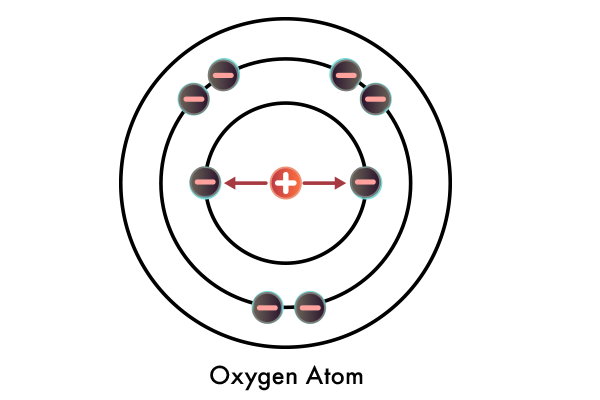
\includegraphics[width=\textwidth,height=\textheight,keepaspectratio]{images/screening-constant}
    \sidecaption{Removing electrons.}
    \label{fig:screening-constant}
\end{marginfigure}

\paragraph{Screening Constant} In general, subtracting the number of shielding (core) electrons (also called the screening constant) from the total nuclear charge (number of protons) gives an estimate of the effective nuclear charge felt by the electrons in an atom's outermost shell.

\begin{marginfigure}
    \centering
    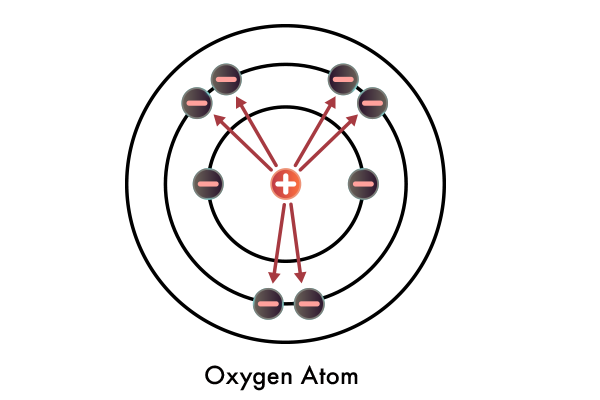
\includegraphics[width=\textwidth,height=\textheight,keepaspectratio]{images/estimating-effective-nuclear-charge}
    \sidecaption{Here is how we estimate the effective nuclear charge.}
    \label{fig:estimating-effective-nuclear-charge}
\end{marginfigure}

\paragraph{Estimating Effective Nuclear Charge} The $+8$ charge of oxygen's nucleus is shielded by the two core electrons in the first energy level. This means each of the outer shell electrons in oxygen feels an estimated effective nuclear charge of about $+6$. This is calculated by:

\begin{align}
    8 - 2 = +6 \\
    \rm{(total nuclear charge) - (shielding electrons) = (effective charge)}
\end{align}

\newpage

\begin{marginfigure}
    \centering
    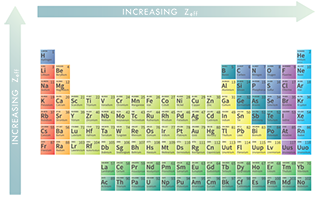
\includegraphics[width=\textwidth,height=\textheight,keepaspectratio]{images/effective-nuclear-charge-across-periods}
    \sidecaption{Periodic Table.}
    \label{fig:effective-nuclear-charge-across-periods}
\end{marginfigure}

\paragraph{Effective Nuclear Charge Across Periods} Across a period:

\begin{itemize}
    \item The overall nuclear charge increases by one with each additional proton.
    \item Each atom also has an additional electron in its outer energy level, but the number of core electrons in the lower energy levels remains the same.
    \item The screening constant stays the same.
\end{itemize}

For instance, phosphorous is to the left of sulfur. It has $15$ protons and $15$ electrons. Like sulfur, it has the same number of electrons in its innermost energy shells, which is $10$.

\begin{align}
    \rm{Sulfur: } z_{eff}         &= +16 - 10 = +6 \\
    \rm{Phosphorus: } z_{eff}     &= +15 - 10 = +5
\end{align}

\begin{marginfigure}
    \centering
    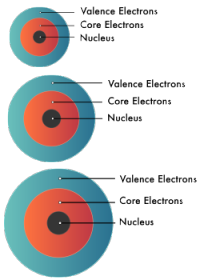
\includegraphics[width=\textwidth,height=\textheight,keepaspectratio]{images/effective-nuclear-charge-down-groups}
    \sidecaption{Electrons in each group.}
    \label{fig:effective-nuclear-charge-down-groups}
\end{marginfigure}

\paragraph{Effective Nuclear Charge Down Groups} The effective nuclear charge felt by an atom's outer shell electrons moving down a group is affected by competing components.

\begin{itemize}
    \item Nucleus
    \item Shielding core Electrons
    \item Outer Shell Electrons
\end{itemize}

\begin{itemize}
    \item Protons increase down a group, causing a greater attraction between protons and outer shell electrons. Electrons are pulled inward toward the nucleus.
    \item The size of atoms and the number of core electrons also increase down a group, thus increasing the number of shielding electrons.
\end{itemize}

Therefore, the nuclear charge of outer shell electrons stays relatively constant for each element down a group. This is because the number of additional protons in each element's nucleus is equal to the number of additional shielding electrons in the inner energy levels of the atom.

For example, \bf{Lithium (Li)}, \bf{Sodium (Na)} and \bf{Potassium (K)} in \it{Group 1} each have an effective nuclear charge of $+1$ felt by its one outer shell electron.

\newpage
